\documentclass[a4paper, 11pt]{article}
\usepackage[english]{babel}
\usepackage[utf8]{inputenc}
\usepackage{amsmath}
\usepackage{amsfonts}
\usepackage{amssymb}
\usepackage{graphicx}
\usepackage{booktabs}
\usepackage{float}
\usepackage{wrapfig}
\usepackage{fixltx2e}
\usepackage{listings}
\usepackage{color}
\usepackage{latexsym}
\usepackage{lstautogobble}
\usepackage[colorinlistoftodos]{todonotes}
\usepackage[margin=3cm]{geometry}
\usepackage{hyperref}
\usepackage{libertine}
\usepackage{tikz}
\usepackage{mathtools, nccmath}
\usepackage{commath}
\hypersetup{
	hidelinks, 
	colorlinks = true,
	linkcolor = black,
}

\usetikzlibrary{patterns}
\usetikzlibrary{shapes,arrows,positioning,calc}
\usetikzlibrary{decorations.pathreplacing}

\newcommand{\N}{\mathbb{N}}
\newcommand{\Exp}{\mathbf{Exp}}
\newcommand{\p}{\mathbf{P}}
\newcommand{\tim}{\mathbf{Time(n)}}
\newcommand{\np}{\mathbf{NP}}
\newcommand{\npc}{\mathbf{NPC}}
\newcommand{\conp}{\mathbf{CO}\text{-}\mathbf{NP}}
\newcommand{\ph}{\mathbf{PH}}
\newcommand{\ntime}{\mathbf{NTIME}}
\newcommand{\nexp}{\mathbf{NEXP}}
\newcommand{\DP}{\mathbf{DP}}
\newcommand{\Space}{\mathbf{SPACE}}
\newcommand{\pspace}{\mathbf{PSPACE}}
\newcommand{\nspace}{\mathbf{NSPACE}}
\newcommand{\npspace}{\mathbf{NPSPACE}}
\newcommand{\apx}{\mathbf{APX}}
\newcommand{\prob}[1]{\mathbb{#1}}
\newcommand{\instance}[1]{\mathcal{I}(\prob{#1})}
\newcommand{\alg}[1]{\mathcal{#1}}
\newcommand{\compl}[2]{T_\alg{#1}( \vert #2 \vert)}
\newcommand{\compld}[3]{T_\alg{#1}( \vert #2 \vert + \vert #3 \vert)}
\newtheorem{thm}{Teorema}[subsection]
\newcommand{\tikzmark}[1]{\tikz[overlay,remember picture,baseline=(#1.base)]
	\node (#1) {\strut};}

\tikzstyle{box} = [rectangle, 
rounded corners, minimum width=1cm, minimum height=1cm,text centered, draw=black]
\begin{document}
	\pagenumbering{gobble}
		\section{Riassunto delle classi di complessità}
	
	\begin{figure}[h!]
		\centering
		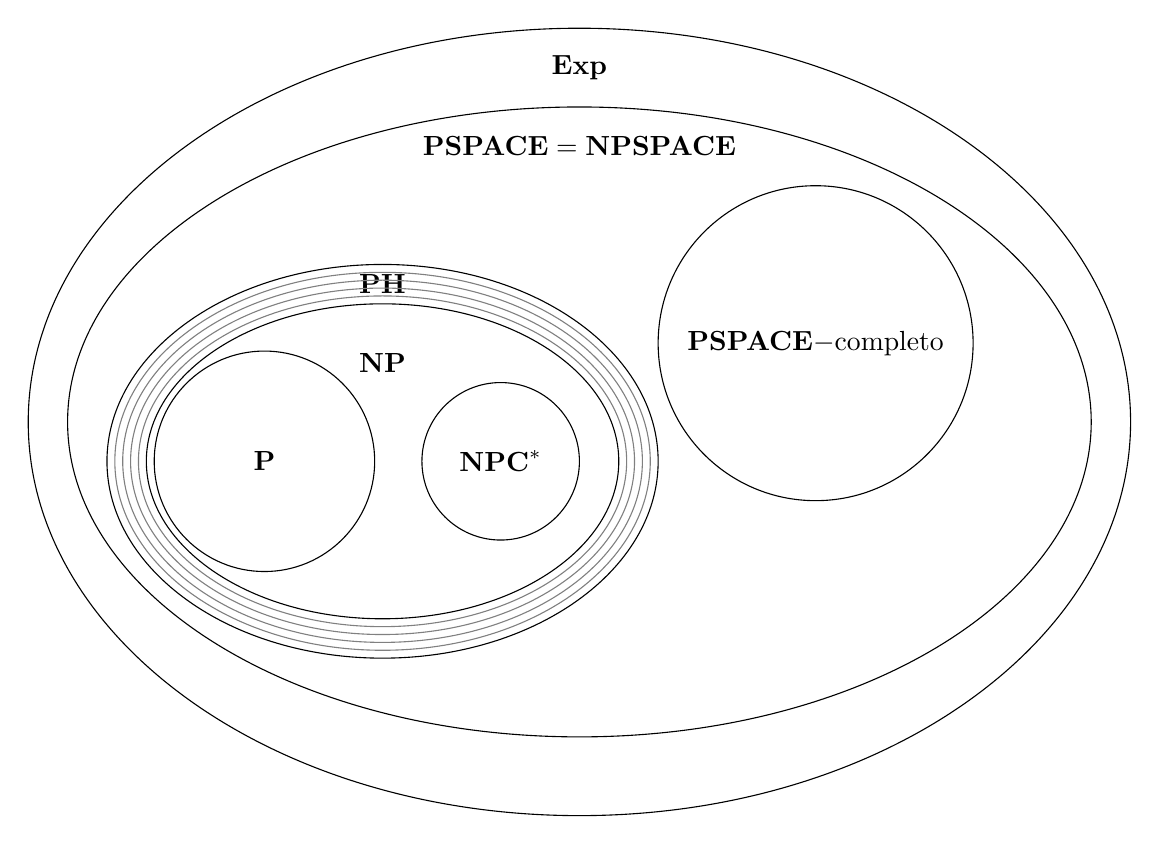
\begin{tikzpicture}
		\draw (0,0) ellipse (7cm and 5cm) node[yshift=4.5cm] {$ \Exp $};
		\draw (0,0) ellipse (6.5cm and 4cm) node[yshift=3.5cm] {$ \pspace = \npspace $};
		\draw (3,1) ellipse (2cm and 2cm) node {$ \pspace-$completo};
		\draw (-2.5,-.5) ellipse (3.5cm and 2.5cm) node[yshift=2.25cm] {$ \ph $};
		\draw[color=gray] (-2.5,-.5) ellipse (3.4cm and 2.4cm);
		\draw[color=gray] (-2.5,-.5) ellipse (3.3cm and 2.3cm);
		\draw[color=gray] (-2.5,-.5) ellipse (3.2cm and 2.2cm);
		\draw[color=gray] (-2.5,-.5) ellipse (3.1cm and 2.1cm);
		\draw (-2.5,-.5) ellipse (3cm and 2cm) node[yshift=1.25cm] {$ \np $};
		\draw (-4,-.5) ellipse (1.4cm and 1.4cm) node {$ \p $};
		\draw (-1,-.5) ellipse (1cm and 1cm) node {$ \npc^{*} $};
		\end{tikzpicture}
	\end{figure}

	
	\section{Classi di complessità in breve}
	\subsection{Temporali}
	\begin{align*}
		\p &= \big\lbrace \mathbb{A}\ |\ \exists B\ t.c.\ \forall x \in J(\mathbb{A}), B(x) = \mathbb{A}(x), B \in O(\abs{x}^c) \big\rbrace \\
		\np &= \big\lbrace \prob{A} \quad \big| \quad \exists \alg{B}(\stackrel{x}{\cdot}, \stackrel{w}{\cdot})\quad t.c.\quad \compld{\alg{B}}{x}{w}= O((\vert x\vert + \vert w\vert)^c) \\
		& \qquad \forall x \in \instance{\prob{A}}\quad \prob{A}(x) = yes\ \Leftrightarrow\ \exists w\ t.c.\quad \vert w \vert = O(\vert x\vert^d)\ \text{ e }\ \alg{B}(x, w) = yes \big\rbrace \\
		\Exp &= \big\lbrace \prob{A}\ \vert\ \exists \alg{A}\ t.c.\ \forall x \in \instance{A},\ \alg{A}(x) = \prob{A}(x)\ \text{ e }\ \compl{A}{x} \leq 2^{\vert x \vert ^ c} \big\rbrace \\
		\mathbf{NP}\text{\textbf{-completo}}\ &= \big\lbrace \exists p(x) = x^k,\ \exists V(\cdot, \cdot) \quad t.c.\quad T_V(a, b) = \mathcal{O}\big(p(|a|+|b|)\big) \\
		&\qquad \text{ e } \ \forall x \in \mathcal{I}(\mathbb{A}),\ \mathbb{A}(x)=yes \Leftrightarrow \exists w \in \{0, 1 \}^{p(|x|)},\ V(x, w)=yes \big\rbrace
	\end{align*}
	\subsection{Spaziali}
	\begin{align*}
		\Space(f(n)) &= \big\lbrace \prob{A}\ \Big|\ \text{ esiste un programma/algoritmo che risolve istanze di } \prob{A} \\ 
		& \qquad \text{usando al più } O(f(n)) \text{ bit di memoria di lavoro e accede }\\
		&\qquad \text{all'istanza in sola lettura. } n \text{ è la taglia dell'istanza}. \big\rbrace \\
		\pspace &= \bigcup\limits_{k > 0} \Space(n^k) \\
			\ntime &= \big\lbrace \prob{A} \ \Big| \ \text{esiste un verificatore } V_{\prob{A}}(\cdot, \cdot) \prob{A} = yes \ \Leftrightarrow\ V_{\prob{A}}(x, w) = yes \\
		& \qquad V_{\prob{A}} \text{ impiega tempo } O(f(\vert x \vert)) \text{ e }\vert w \vert = O(f(\vert x \vert)) \ \big\rbrace \\
		\nspace &= \big\lbrace  \prob{A}\ \Big| \ \text{ esiste un algoritmo/programma } \Pi \text{ \textit{non deterministico}} \\
		& \qquad \text{che risolve } x \in \instance{A} \text{ usando memoria di lavoro } O(f(\vert x\vert)) \quad \Pi(x) = \prob{A}(x) \ \big\rbrace \\
		\npspace &= \bigcup\limits_{k > 0} \nspace(n^k) \\
		\pspace\text{-completo} &=\begin{cases}
		 \prob{A} \in \pspace  \\
		 \forall \prob{B} \in \pspace \quad \prob{B} \leq_K \prob{A} \  (\text{hardness}) \\
		\end{cases}\\
	\end{align*}
	
	\section{Teoremi vari}
	\begin{thm}[Teorema di Savitch]
		Per ogni funzione $f(n) \geq log(n)$ vale \\ $ \nspace(f(n)) \leq \Space(f(n)^2) $
	\end{thm}

	\begin{thm}[Teorema di Ladner]
		Se $\p \neq \np$ allora esiste un problema $\mathbb{A}$ tale che $\prob{A} \in \np \setminus (\p \cup \npc)$
	\end{thm}

	\begin{thm}[Self-reducibility]
					$ \prob{A}\in \np $ (rispetto a $ V_{\prob{A}} $) è \textbf{self reducible} se, dato un \textbf{oracolo} per il problema di decisione-$\prob{A} $, esiste un algoritmo polinomiale per il problema di ricerca-$\prob{A} $. Ogni problema $\npc$ è self-reducible.
	\end{thm}
	
	\newpage
	\section{Lista dei problemi visti e complessità}
	\begin{figure}[h!]
		\begin{tabular}{lccccccc}
			\toprule
			\textbf{Problema} & {\small $ \p $} & {\small $ \np $} & {\small $ \npc $} & {\small $ \conp\mathbf{C} $} & {\small $ \pspace $} & {\small $ \pspace$-compl} & {\small \textbf{Riduzione da}}\\
			\midrule
			Eulerian Cycle & \checkmark & & & & \checkmark & & \\
			K-Colouring (K=2) & \checkmark & & & & \checkmark & & \\
			K-Colouring (K $>$ 2) & & \checkmark & \checkmark & & \checkmark & & ($ \leq_K $) (K+1)-Col  \\
			K-SAT (K=2) & \checkmark & & & & \checkmark & & \\
			K-SAT (K $>$ 2) & & \checkmark & \checkmark & & \checkmark & & K-Colouring\\
			Circuit-SAT & & \checkmark & \checkmark & & \checkmark &  & ($ \leq_K $) SAT\\
			Tautology & & & & \checkmark & \checkmark & & \\
			Min-Circuit Bool\footnotemark[1] & & & & & \checkmark & & \\
			Graph Isomorphism & & \checkmark & & & \checkmark & & \\
			Clique & & \checkmark & \checkmark & & \checkmark & & 3-SAT \\
			Clique-no-Clique & & \checkmark & \checkmark & & \checkmark & & $ \prob{A}\in\mathbf{DP} $\\
			Independent Set & & \checkmark & \checkmark & & \checkmark & & Clique \\
			Only Small IndSet & & & & \checkmark & \checkmark & & \\
			Vertex Cover & & \checkmark & \checkmark & & \checkmark & & Independent Set\\
			Hitting Set & & \checkmark & \checkmark & & \checkmark & & Vertex Cover \\
			Max Cut & & \checkmark & \checkmark & & \checkmark & & NAE-3-SAT\\
			Set Splitting & & \checkmark & \checkmark & & \checkmark & & NAE-3-SAT\\
			Set Cover & & \checkmark & \checkmark & & \checkmark & & Vertex Cover\\
			Hamiltonian Path & & \checkmark & \checkmark & & \checkmark & &  \\

			Q-SAT (= 2p-SAT) & & & & & & \checkmark &  \\
			Geography & & & & & & \checkmark & Q-SAT\\
			Alternating Hampath & & & & & & \checkmark & Q-SAT \\
			Reachability\footnotemark[2] & \checkmark & & & & \checkmark & & \\
			Makespan-m & & \checkmark & \checkmark & & \checkmark & &  Partition\\
			SubsetSum & & \checkmark & \checkmark & & \checkmark & & \\
			Partition & & \checkmark & \checkmark & & \checkmark & & \\
			Traveling Salesman & & \checkmark & \checkmark & & \checkmark & & HamCycle\\
			Knapsack & & \checkmark & \checkmark & & \checkmark & & Partition\\
			Max-k-xor-SAT & & \checkmark & \checkmark & & \checkmark & & \\
			Max-k-SAT & & \checkmark & \checkmark & & \checkmark & & Max Cut\\
			Set Cover & & \checkmark & \checkmark & & \checkmark & & Vertex Cover\\
			\bottomrule
		\end{tabular}
	\end{figure}
\end{document}